% !TEX root = ../Thesis.tex
\chapter{Introduction}
\label{c:intro}

Within the last decades, data has not only grown in volume and variety but also in importance throughout every industry. 
Whereas data has so far only been considered a mere tool to assist certain tasks, it developed towards inherently
driving new technologies and scientifc advancements, becoming an industry focus-point on its own ~\cite{data-driven_2014}.\\
To process the ever-increasing volume and complexity of the data, companies nowadays do not only rely on their data by itself but utilize 
all forms of data ingestion methods to extract and connect nested knowledge out of different sources 
to gain economical advantages by prediciting new trends ~\cite{ingestion_2016}.\\
However, this also increased the need to reliably store and rapidly access such information, along constantly varying requirements.
Database management systems (DBMS) are therefore progressively challenged, to handle these swiftly growing heterogeneous datasets as efficiently as possible,
while being able to adapt to new situations. 
To meet these new demands and consequently process and extract meaningful information required by data-driven applications, new systems have emerged.\\
To improve the overall data retrieval time, these novel Polystore systems natively combine different physical data engines to 
adapt to different workloads by leveraging the key benefits of each underlying engine ~\cite{stonebraker:2005, polypheny2020}. 
Although such systems are inherently built to process heterogeneous data with high throughput, they still need to adhere to the given requirements
and store all data reliably to protect it against failures.\\
Especially since cloud computing has become a crucial and central part with regards to data processing, 
companies tend to progressively store and manage their data across different distributed data centers world wide ~\cite{claremont:2005}. 
The access to these storages is provided according to the Service Level Agreement (SLA) of the respective provider.
Such quality guarantees usually include elastic up- and down-scaling of resources as well as a high degree of availability.
This can ulitmately be achieved by replicating data throughout different regions, to provide resilient and fault tolerant architectures ~\cite{brinkmann:2015, terry:2013}.\\
However, in order to safely manage these large distributed volumes of data, it needs to be replicated eagerly to 
every particpating node to ensure a global data consistency and avoid losing data. 
This however impacts the accesibility of a node and reduces the possibility to be parallelly used for read access.

Therefore, cloud providers need to design their services 
to balance between a sufficient protection against failures and still providing adequate access times to the data ~\cite{cap2002, levandowski2013}.
To support varying use cases, data freshness strategies were introduced as an essential part of distributed data management systems.\\
The freshness essentially corresponds to the age of a specific data item and reflects how current and up-to-date it is.
Because they might pursue different goals and data is not always equally important to depending applications, they can often tolerate different levels of freshness.
Especially for analytical queries, that often spend hours retrieving, extracting and combining relevant data, slightly outdated data will not drastically 
impact the final result.\\
This consequently allows to lower the constraints to replicate data only to a subset of nodes and still efficiently 
utilizing the remaining resources to be used for data retrieval.


%%%%%%%%%%%%%%%%%%%%%%%%%%%%%%%%%%%%%%%%%%%%%%%%%%%%%%%%%%%%%%%%%%


\section{Polystores}

The decission which data structure to use has a fundamental impact on the overall performance of a system~\cite{plattner2015}.\\
While row-oriented data stores might be useful and preferred for write-heavy transactional 
workloads, they are rather insufficient for purely analytical workload which would rather benefit from a
column-oriented data store with less write operations ~\cite{sigmond2008}.\\

Despite the fact that a variety of DBMS exist which were originally created with an intention to support specific scenarios,
applications are getting more complex relying on various requirements and characteristics to serve multiple use cases at once.
That is why modern day applications can not solely rely on one storage technology alone. 
Consequently Multi- and Polystore systems have emerged. \\
\\
While multistore database systems aim to combine and manage data across heterogeneous data stores,
polystore systems are essentially based on the idea of combining multistores with
\textit{polyglot persistence} ~\cite{polypheny2020}.
Polyglot persistence is a term which refers to a practice originated from the concept 
of \textit{polyglot programming}, to utilize different 
programming languages for different tasks following a best-fit approach ~\cite{fowler2011}. \\
Along this paradigm, polystores want to utilize multiple data storage technologies to
fulfill different needs for different application components in order to cope
with mixed and varying workloads.

%%%%%%%%%%%%%%%%%%%%%%%%%%%%%%%%%%%%%%%%%%%%%%%%%%%%%%%%%%%%%%%%%%

\section{Motivation}

Due to the growth in data and complexity, polystore systems aim to provide fast response times for various use cases and applications of all kind.
These systems natively encompass several different stores, where each is capable of fulfilling a different requirement. 
This enables an application to harvest the best possible response times for different workloads.
Because polystore systems orginally were introduced to support heterogenous data, they mostly do this by utilizing different stores at once.
Since these systems are inherently distributed the data will be stored redundantly across these stores. 
In order for such systems to utilize the different underlying engines and consequently improve the read-performance, 
the data also needs to be consistently written to all relevant stores to leverage their unique benefits.
This however, limits the performance of such write-operations essentially to be bound to the slowest performing node in such a setup \todoMissing{figure}.

\begin{figure}[t] 
    \centering 
    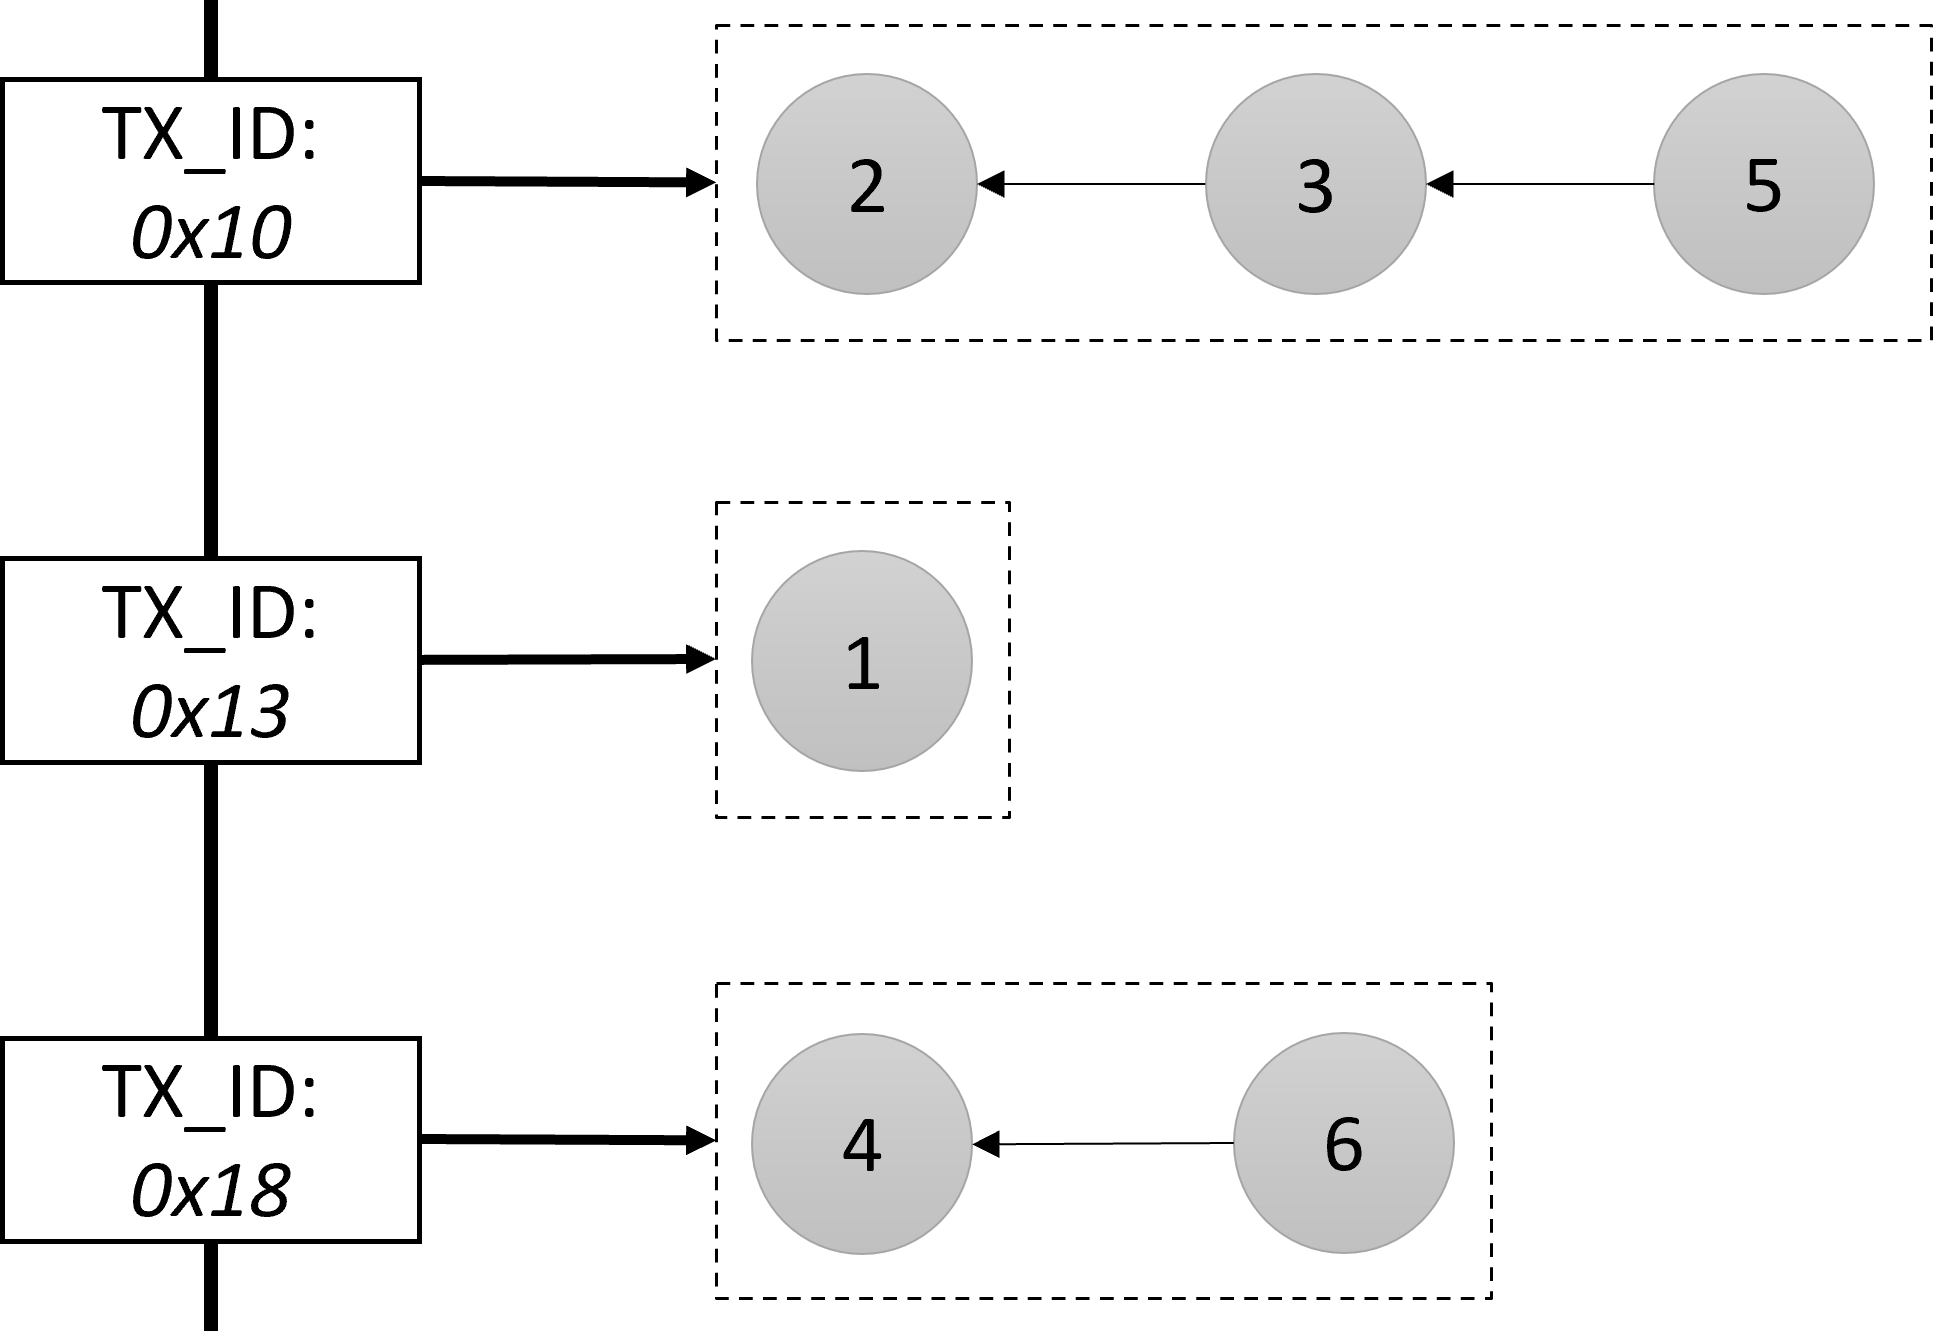
\includegraphics[width=0.7\textwidth]{Figures/store_comparision.png}
    \caption{Execution-Time comparision of a single write-operation on different stores.}
    \label{fig:store_comparision}
\end{figure}
 
As depicted in Figure \ref{fig:store_comparision}, the utilized stores write the same data very differently, leading to large deviations in their execution time. 
This negativiely impacts the overall performance of such systems.
Additionally this might also reduce the availability of the entire system, since it might not allow read-operations to be executed in parallel. 
But again since these stores differ in terms of there field of application we cannot simply remove the slower performing stores to improve write operations. 
This would comprehensively neglect all benefits originally introduced by polystore systems.
Essentially the system needs to be able to allow transactional as well as analytical workload to be executed in parallel.\\
This could be accomplished by decoupling updates on a system to only target specific stores. These stores can then be used to asynchronously update
the remaining stores without directly affecting the user with obsolete wait-situations.\\
Although, reducing the consistency of the system, this approach intuitively generates multiple temporary versions per data object.
In order to efficiently utilize the resources of the entire system users or applications can choose to query these versions by
considering their \emph{freshness}.
Since some requests do not always require the most recent data, the maximum tolerated degree of outdatedness could be specified during retrieval.
This specification could then be used to identify a well-suited location to retrieve the desired data object. 
This notion of freshness aids to efficiently use these temporary outdated versions for reads as well. 
Hence it allows the system to execute read- and write-operations in parallel.
Further it mitigates the need to immediately update every existing data replica to the most recent state.
Such delayed updates now allow for a much higher throughput and increased performance in scenarios were also slightly 
outdated data is acceptable.\\
On the basis of polystore systems we could now use this scenario to nativiely leverage the benefit of a heavily write-optimized store to 
primarly receive any write-operation.
Which then distributes the received changes asnychronously to the remaining stores, and
would immediately allow using the notion of freshness to be able to utilize outdated data.
This would ultimately loosen the constraints and downsides of polystore systems to efficiently utilize all available resources



%%%%%%%%%%%%%%%%%%%%%%%%%%%%%%%%%%%%%%%%%%%%%%%%%%%%%%%%%%%%%%%%%%

\section{Contribution}
The contribution of this thesis is fivefold. First, we identify and define the necessary requirements to establish freshness-awareness in general.
Second, we outline and propose various possibilities to enable freshness-awareness within a DBMS. Third, we reduce the existing locking constraints and 
introduce a fault-tolerant replication algorithm, to automatically refresh outdated stores within Polypheny-DB. 
Fourth, we establish a query extension to allow the specification of tolerated and desirable freshness levels 
on various metrics. Fifth, we adapt the routing system to use those freshness constraints to efficiently identify and route queries towards the appropriate stores, 
to allow the possibility to decouple primary from secondary transactions.



%%%%%%%%%%%%%%%%%%%%%%%%%%%%%%%%%%%%%%%%%%%%%%%%%%%%%%%%%%%%%%%%%%

\section{Outline}
This thesis is structured as follows:
In Chapter \ref{c:related} the foundations and concepts of data freshness characteristics and requirements are presented.
Further, we give an overview over the current state of research in the field of data freshness. 
Chapter \ref{c:Foundation} illustrates existing fundamental concepts in the context of distributed data management systems. 
Followed by Chapter \ref{c:concept} which describes the functional requirements, necessary to introduce the notion of freshness inside a polystore system. 
Additionally, it discusses and proposes possible approaches how to implement them in a polystore system. 
In Chapter \ref{c:implementation} these concepts including all requirements and building blocks will be applied to Polypheny-DB, a specific polystore system.
While Chapter \ref{c:evaluation} focuses on possibilities how to ensure correctness and measure the performance of the implementation, including all necessary prerequisites.
Finally, Chapter \ref{c:conclusion} concludes the thesis by summarizing the individual contributions according to the proposed
implementations and gives an outlook to future work and possible extensions.


